% ==============================================================================
\chapter{Discretization: Isogeometric Analysis (IGA)}
\label{ch:discretization}
% ==============================================================================

\section{Geometric Representation via B-Splines and NURBS}
Isogeometric Analysis (IGA) utilizes the same mathematical basis functions to represent the physical geometry and to approximate the field variables. This maintains exact geometric descriptions throughout the analysis process and allows for shape parameterization without approximation errors. The concept and theoretical foundations of Isogeometric Analysis, bridging the gap between Computer-Aided Design (CAD) and Finite Element Analysis (FEA), were pioneered by Hughes et al.~\cite{hughes2005} and are detailed extensively in the seminal textbook~\cite{cottrell2009}.

\subsection{B-Spline Basis Functions}
Evaluating B-spline basis functions is performed over an open knot vector $\Xi = \{\xi_0, \xi_1, \dots, \xi_{m}\}$ where $m = n + p + 1$, $p$ is the polynomial degree, and $n$ is the number of basis functions. The recursive Cox-de Boor formula defines the basis functions $N_{i,p}(\xi)$ as:
\begin{equation}
    N_{i,0}(\xi) = \begin{cases} 1 & \text{if } \xi_i \le \xi < \xi_{i+1} \\ 0 & \text{otherwise} \end{cases}
\end{equation}
\begin{equation}
    N_{i,p}(\xi) = \frac{\xi - \xi_i}{\xi_{i+p} - \xi_i} N_{i,p-1}(\xi) + \frac{\xi_{i+p+1} - \xi}{\xi_{i+p+1} - \xi_{i+1}} N_{i+1,p-1}(\xi)
\end{equation}
with the convention $0/0 = 0$.

For structural mechanics applications where variational strain energies involve spatial derivatives, the gradients of the basis functions are evaluated using the analytical derivative recurrence:
\begin{equation}
    \frac{d}{d\xi} N_{i,p}(\xi) = p \left( \frac{N_{i,p-1}(\xi)}{\xi_{i+p} - \xi_i} - \frac{N_{i+1,p-1}(\xi)}{\xi_{i+p+1} - \xi_{i+1}} \right)
\end{equation}

\subsection{Non-Uniform Rational B-Splines (NURBS)}
To represent conic sections or complex parameterized boundaries exactly, projective control weights $w_i$ are injected, defining the rational basis functions $R_{i,p}(\xi)$ as:
\begin{equation}
    R_{i,p}(\xi) = \frac{N_{i,p}(\xi) w_i}{\sum_{j=0}^{n-1} N_{j,p}(\xi) w_j}
\end{equation}

The spatial gradients of the rational basis functions are evaluated using the quotient rule:
\begin{equation}
    \frac{d}{d\xi} R_{i,p}(\xi) = w_i \frac{\frac{d N_{i,p}(\xi)}{d\xi} W(\xi) - N_{i,p}(\xi) \frac{d W(\xi)}{d\xi}}{[W(\xi)]^2}
\end{equation}
where $W(\xi) = \sum_{j=0}^{n-1} N_{j,p}(\xi) w_j$ is the denominator projective sum function. The physical coordinates of a 1D parametric curve $\vect{C}(\xi)$ are given by:
\begin{equation}
    \vect{C}(\xi) = \sum_{i=0}^{n-1} R_{i,p}(\xi) \vect{P}_i
\end{equation}
where $\vect{P}_i$ are the coordinates of the control points.

\begin{figure}[htbp]
    \centering
    \makebox[\textwidth][c]{%
        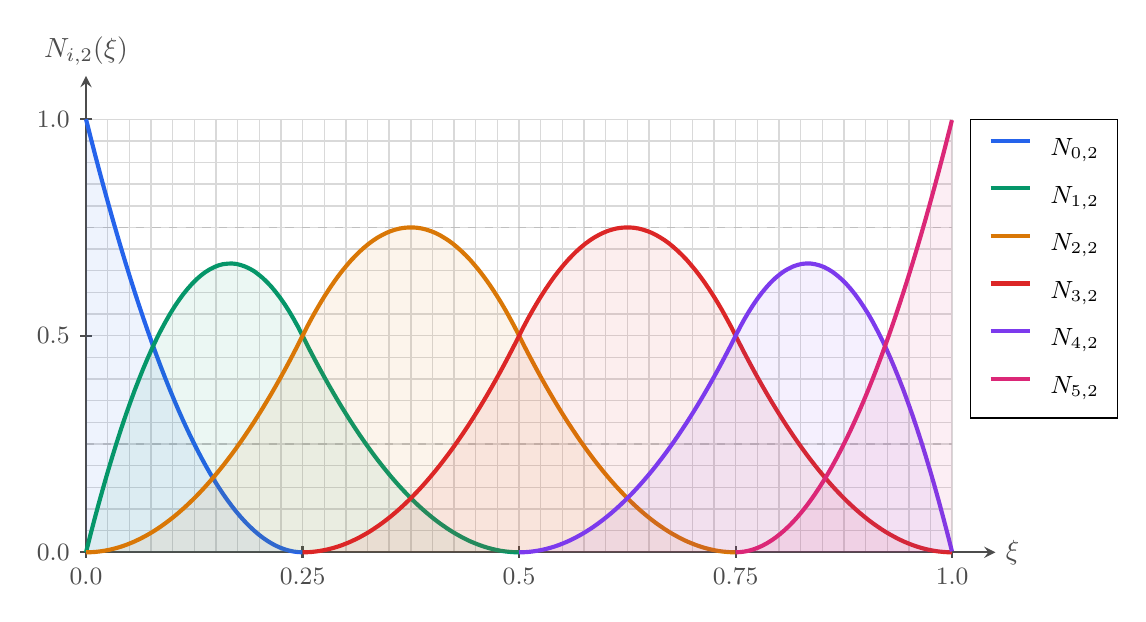
\begin{tikzpicture}[scale=1.1, >=stealth]
            % Define Colors matching the theme
            \definecolor{n0color}{RGB}{37, 99, 235}   % Blue
            \definecolor{n1color}{RGB}{5, 150, 105}   % Green
            \definecolor{n2color}{RGB}{217, 119, 6}   % Orange
            \definecolor{n3color}{RGB}{220, 38, 38}   % Red
            \definecolor{n4color}{RGB}{124, 58, 237}  % Purple
            \definecolor{n5color}{RGB}{219, 39, 119}  % Pink/Magenta

            % Grid and Axes
            \draw[gray!30, line width=0.5pt] (0, 0) grid[ystep=0.25, xstep=0.25] (10, 5);
            \draw[gray!50, dashed, line width=0.5pt] (0, 1.25) -- (10, 1.25);
            \draw[gray!50, dashed, line width=0.5pt] (0, 3.75) -- (10, 3.75);

            % Axes lines
            \draw[->, thick, black!70] (0,0) -- (10.5,0) node[right] {$\xi$};
            \draw[->, thick, black!70] (0,0) -- (0,5.5) node[above] {$N_{i,2}(\xi)$};

            % X-Ticks
            \foreach \x/\label in {0/0.0, 2.5/0.25, 5/0.5, 7.5/0.75, 10/1.0} {
                    \draw[black!70, thick] (\x, 2pt) -- (\x, -2pt) node[below, font=\small] {\label};
                }
            % Y-Ticks
            \foreach \y/\label in {0/0.0, 2.5/0.5, 5/1.0} {
                    \draw[black!70, thick] (2pt, \y) -- (-2pt, \y) node[left, font=\small] {\label};
                }

            % --- PLOTS AND FILLS ---
            % Scale factor: x goes from 0 to 10 (scale=10), y goes from 0 to 5 (scale=5)

            % N_{0,2} (Blue)
            \fill[n0color, opacity=0.08] (0,5) -- plot[domain=0:0.25, samples=50] ({10*\x}, {5*(1-4*\x)^2}) -- (2.5,0) -- (0,0) -- cycle;
            \draw[n0color, line width=1.5pt] plot[domain=0:0.25, samples=50] ({10*\x}, {5*(1-4*\x)^2});

            % N_{1,2} (Green)
            \fill[n1color, opacity=0.08] (0,0) -- plot[domain=0:0.25, samples=50] ({10*\x}, {5*(8*\x - 24*\x^2)}) -- plot[domain=0.25:0.5, samples=50] ({10*\x}, {5*(8*(0.5-\x)^2)}) -- (5,0) -- cycle;
            \draw[n1color, line width=1.5pt] plot[domain=0:0.25, samples=50] ({10*\x}, {5*(8*\x - 24*\x^2)}) -- plot[domain=0.25:0.5, samples=50] ({10*\x}, {5*(8*(0.5-\x)^2)});

            % N_{2,2} (Orange)
            \fill[n2color, opacity=0.08] (0,0) -- plot[domain=0:0.25, samples=50] ({10*\x}, {5*(8*\x^2)}) -- plot[domain=0.25:0.5, samples=50] ({10*\x}, {5*(12*\x - 16*\x^2 - 1.5)}) -- plot[domain=0.5:0.75, samples=50] ({10*\x}, {5*(8*(0.75-\x)^2)}) -- (7.5,0) -- cycle;
            \draw[n2color, line width=1.5pt] plot[domain=0:0.25, samples=50] ({10*\x}, {5*(8*\x^2)}) -- plot[domain=0.25:0.5, samples=50] ({10*\x}, {5*(12*\x - 16*\x^2 - 1.5)}) -- plot[domain=0.5:0.75, samples=50] ({10*\x}, {5*(8*(0.75-\x)^2)});

            % N_{3,2} (Red)
            \fill[n3color, opacity=0.08] (2.5,0) -- plot[domain=0.25:0.5, samples=50] ({10*\x}, {5*(8*(\x-0.25)^2)}) -- plot[domain=0.5:0.75, samples=50] ({10*\x}, {5*(12*(1-\x) - 16*(1-\x)^2 - 1.5)}) -- plot[domain=0.75:1.0, samples=50] ({10*\x}, {5*(8*(1-\x)^2)}) -- (10,0) -- cycle;
            \draw[n3color, line width=1.5pt] plot[domain=0.25:0.5, samples=50] ({10*\x}, {5*(8*(\x-0.25)^2)}) -- plot[domain=0.5:0.75, samples=50] ({10*\x}, {5*(12*(1-\x) - 16*(1-\x)^2 - 1.5)}) -- plot[domain=0.75:1.0, samples=50] ({10*\x}, {5*(8*(1-\x)^2)});

            % N_{4,2} (Purple)
            \fill[n4color, opacity=0.08] (5,0) -- plot[domain=0.5:0.75, samples=50] ({10*\x}, {5*(8*(\x-0.5)^2)}) -- plot[domain=0.75:1.0, samples=50] ({10*\x}, {5*(8*(1-\x) - 24*(1-\x)^2)}) -- (10,0) -- cycle;
            \draw[n4color, line width=1.5pt] plot[domain=0.5:0.75, samples=50] ({10*\x}, {5*(8*(\x-0.5)^2)}) -- plot[domain=0.75:1.0, samples=50] ({10*\x}, {5*(8*(1-\x) - 24*(1-\x)^2)});

            % N_{5,2} (Pink)
            \fill[n5color, opacity=0.08] (7.5,0) -- plot[domain=0.75:1.0, samples=50] ({10*\x}, {5*(4*\x-3)^2}) -- (10,5) -- (10,0) -- cycle;
            \draw[n5color, line width=1.5pt] plot[domain=0.75:1.0, samples=50] ({10*\x}, {5*(4*\x-3)^2});

            % Legend
            \matrix [draw, fill=white, at={(10.2, 5)}, anchor=north west, font=\small, row sep=2pt, ampersand replacement=\&] {
                \node {\tikz[baseline=-0.5ex]{\draw[n0color, line width=1.5pt] (0,0) -- (0.5,0);}}; \& \node {$N_{0,2}$}; \\
                \node {\tikz[baseline=-0.5ex]{\draw[n1color, line width=1.5pt] (0,0) -- (0.5,0);}}; \& \node {$N_{1,2}$}; \\
                \node {\tikz[baseline=-0.5ex]{\draw[n2color, line width=1.5pt] (0,0) -- (0.5,0);}}; \& \node {$N_{2,2}$}; \\
                \node {\tikz[baseline=-0.5ex]{\draw[n3color, line width=1.5pt] (0,0) -- (0.5,0);}}; \& \node {$N_{3,2}$}; \\
                \node {\tikz[baseline=-0.5ex]{\draw[n4color, line width=1.5pt] (0,0) -- (0.5,0);}}; \& \node {$N_{4,2}$}; \\
                \node {\tikz[baseline=-0.5ex]{\draw[n5color, line width=1.5pt] (0,0) -- (0.5,0);}}; \& \node {$N_{5,2}$}; \\
            };

        \end{tikzpicture}%
    }
    \caption{Continuous evaluation of quadratic B-spline basis functions $N_{i,2}(\xi)$ over the knot vector $\Xi = \{0, 0, 0, 0.25, 0.5, 0.75, 1, 1, 1\}$.}
    \label{fig:nurbs_curves_eval}
\end{figure}

\begin{figure}[htbp]
    \centering
    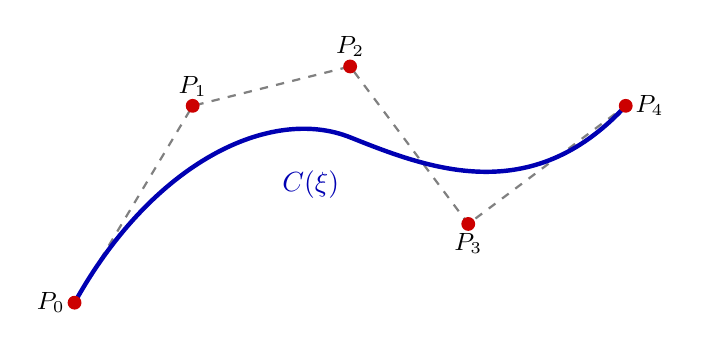
\begin{tikzpicture}[scale=1.0, >=stealth]
        % Control points coordinates
        \coordinate (P0) at (0, 0);
        \coordinate (P1) at (1.5, 2.5);
        \coordinate (P2) at (3.5, 3.0);
        \coordinate (P3) at (5.0, 1.0);
        \coordinate (P4) at (7.0, 2.5);

        % Draw control polygon (dashed)
        \draw[thick, gray, dashed] (P0) -- (P1) -- (P2) -- (P3) -- (P4);

        % Draw actual B-spline curve
        \draw[ultra thick, blue!70!black] (P0) .. controls (1.0,1.8) and (2.5,2.5) .. (3.5,2.1) .. controls (4.5,1.7) and (5.8,1.2) .. (P4);

        % Draw control points
        \foreach \p/\l/\pos in {P0/P_0/left, P1/P_1/above, P2/P_2/above, P3/P_3/below, P4/P_4/right} {
                \fill[red!80!black] (\p) circle (2.5pt);
                \node[\pos, font=\small] at (\p) {$\vect{\l}$};
            }

        % Labels
        \node[blue!70!black, above] at (3, 1.2) {$\vect{C}(\xi)$};
    \end{tikzpicture}
    \caption{Concept of a 1D B-spline curve $\vect{C}(\xi)$ showing the control points $\vect{P}_i$ (red dots) and the dashed control polygon guiding the smooth curve (blue line).}
    \label{fig:bspline_curve_concept}
\end{figure}

Unlike standard Lagrangian finite elements, NURBS basis functions do not possess the Kronecker delta property at internal nodes. Consequently, a control point $\vect{P}_i$ does not represent the physical state at a specific coordinate unless it lies on a repeated boundary knot of multiplicity $p+1$, where the curve interpolates the control point directly.

\subsection{Tensor-Product Bivariate NURBS Mapping Core}
To model 2D structural domains such as the cantilever beam, the geometric representation is extended to two-dimensional manifolds. This is achieved by constructing a tensor product of univariate B-spline basis functions over two independent parametric directions governed by the knot vectors $\Xi = \{\xi_0, \xi_1, \dots, \xi_{r}\}$ and $\mathcal{H} = \{\eta_0, \eta_1, \dots, \eta_{s}\}$, with corresponding polynomial degrees $p$ and $q$.

The bivariate rational basis functions $R_{i,j}^{p,q}(\xi, \eta)$ are formulated by projecting a grid of control weights $w_{i,j}$ across the product space:
\begin{equation}
    R_{i,j}^{p,q}(\xi, \eta) = \frac{N_{i,p}(\xi) M_{j,q}(\eta) w_{i,j}}{\sum_{k=0}^{n-1} \sum_{l=0}^{m-1} N_{k,p}(\xi) M_{l,q}(\eta) w_{k,l}}
\end{equation}
where $N_{i,p}(\xi)$ and $M_{j,q}(\eta)$ represent the standard univariate basis polynomials evaluated along the $\xi$ and $\eta$ directions, respectively. The continuous geometric mapping of the 2D surface patch $\vect{S}(\xi, \eta)$ is expressed as a linear combination of a bidimensional control point lattice $\vect{P}_{i,j} = [x_{i,j}, y_{i,j}, z_{i,j}]^T$:
\begin{equation}
    \vect{S}(\xi, \eta) = \sum_{i=0}^{n-1} \sum_{j=0}^{m-1} R_{i,j}^{p,q}(\xi, \eta) \vect{P}_{i,j}
\end{equation}

\begin{figure}[htbp]
    \centering
    \makebox[\textwidth][c]{%
        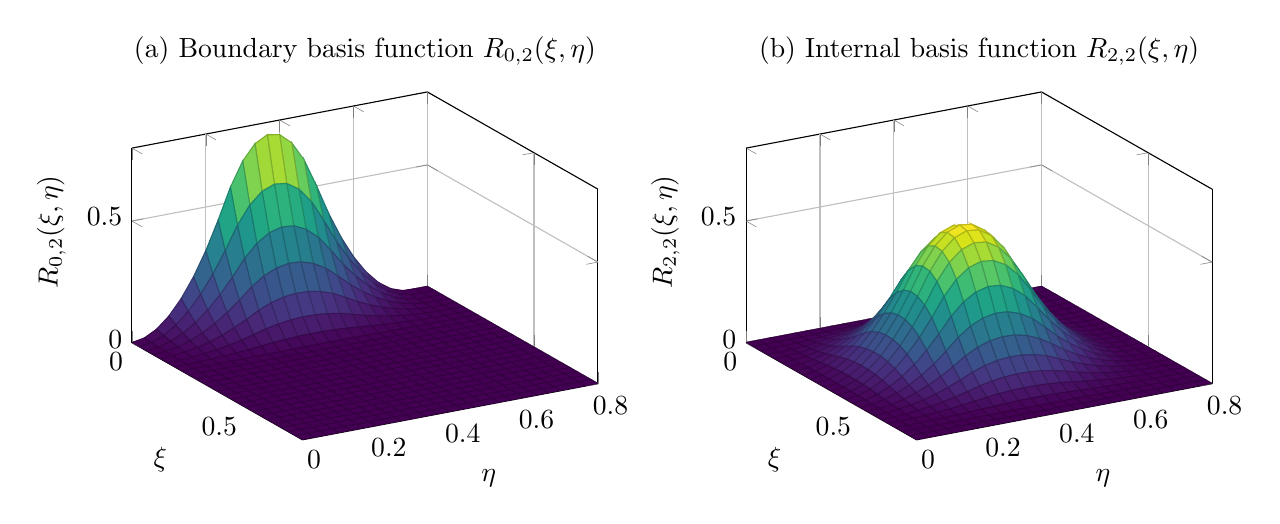
\begin{tikzpicture}[
                declare function={
                        n0(\t) = (\t < 0.25) * ((1-4*\t)^2);
                        n2(\t) = (\t < 0.25) * (8*\t^2) +
                        (\t >= 0.25) * (\t < 0.5) * (12*\t - 16*\t^2 - 1.5) +
                        (\t >= 0.5) * (\t < 0.75) * (8*(0.75-\t)^2);
                    }
            ]
            % Panel (a) Axis
            \begin{axis}[
                    at={(0,0)},
                    width=7.5cm,
                    height=6.0cm,
                    grid=major,
                    xlabel={$\xi$},
                    ylabel={$\eta$},
                    zlabel={$R_{0,2}(\xi,\eta)$},
                    colormap/viridis,
                    view={60}{30},
                    zmin=0, zmax=0.8,
                    title={(a) Boundary basis function $R_{0,2}(\xi,\eta)$}
                ]
                \addplot3[
                    surf,
                    domain=0:0.8,
                    domain y=0:0.8,
                    samples=25,
                    shader=faceted
                ] {n0(x)*n2(y)};
            \end{axis}

            % Panel (b) Axis
            \begin{axis}[
                    at={(7.8cm,0)},
                    width=7.5cm,
                    height=6.0cm,
                    grid=major,
                    xlabel={$\xi$},
                    ylabel={$\eta$},
                    zlabel={$R_{2,2}(\xi,\eta)$},
                    colormap/viridis,
                    view={60}{30},
                    zmin=0, zmax=0.8,
                    title={(b) Internal basis function $R_{2,2}(\xi,\eta)$}
                ]
                \addplot3[
                    surf,
                    domain=0:0.8,
                    domain y=0:0.8,
                    samples=25,
                    shader=faceted
                ] {n2(x)*n2(y)};
            \end{axis}
        \end{tikzpicture}%
    }
    \caption{3D surface plots of two distinct bivariate tensor-product B-spline basis functions: (a) boundary basis function $R_{0,2}(\xi,\eta) = N_{0,2}(\xi)M_{2,2}(\eta)$ and (b) internal basis function $R_{2,2}(\xi,\eta) = N_{2,2}(\xi)M_{2,2}(\eta)$, demonstrating the difference between edge-supported and fully internal support.}
    \label{fig:bivariate_basis_3d}
\end{figure}

\begin{figure}[htbp]
    \centering
    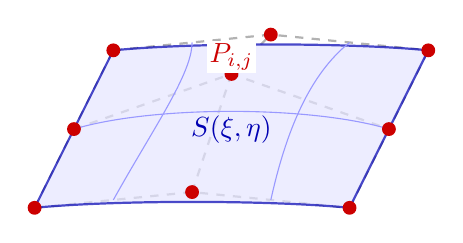
\begin{tikzpicture}[scale=1.0, >=stealth]
        % Row 0 (bottom)
        \coordinate (P00) at (0, 0);
        \coordinate (P10) at (2, 0.2);
        \coordinate (P20) at (4, 0);
        % Row 1 (middle)
        \coordinate (P01) at (0.5, 1.0);
        \coordinate (P11) at (2.5, 1.7); % raised in the middle
        \coordinate (P21) at (4.5, 1.0);
        % Row 2 (top)
        \coordinate (P02) at (1.0, 2.0);
        \coordinate (P12) at (3.0, 2.2);
        \coordinate (P22) at (5.0, 2.0);

        % Draw control net (dashed grid)
        \draw[thick, gray!60, dashed] (P00) -- (P10) -- (P20);
        \draw[thick, gray!60, dashed] (P01) -- (P11) -- (P21);
        \draw[thick, gray!60, dashed] (P02) -- (P12) -- (P22);
        \draw[thick, gray!60, dashed] (P00) -- (P01) -- (P02);
        \draw[thick, gray!60, dashed] (P10) -- (P11) -- (P12);
        \draw[thick, gray!60, dashed] (P20) -- (P21) -- (P22);

        % Draw the smooth surface patch (colored patch)
        \fill[blue!10, opacity=0.7, draw=blue!70!black, thick]
        (P00) .. controls (1.0, 0.1) and (3.0, 0.1) .. (P20)
        .. controls (4.3, 0.6) and (4.7, 1.4) .. (P22)
        .. controls (4.0, 2.1) and (2.0, 2.1) .. (P02)
        .. controls (0.7, 1.4) and (0.3, 0.6) .. (P00);

        % Draw grid lines on the surface patch to show parameter lines
        \draw[blue!40, thin] (1.0, 0.1) .. controls (1.5, 1.0) and (2.0, 1.7) .. (2.0, 2.1);
        \draw[blue!40, thin] (3.0, 0.1) .. controls (3.2, 1.0) and (3.5, 1.7) .. (4.0, 2.1);
        \draw[blue!40, thin] (0.5, 1.0) .. controls (1.5, 1.3) and (3.5, 1.3) .. (4.5, 1.0);

        % Draw control points
        \foreach \p in {P00, P01, P02, P10, P11, P12, P20, P21, P22} {
                \fill[red!80!black] (\p) circle (2.5pt);
            }

        \node[red!80!black, above, fill=white, inner sep=1pt] at (P11) {$\vect{P}_{i,j}$};
        \node[blue!70!black] at (2.5, 1.0) {$\vect{S}(\xi,\eta)$};
    \end{tikzpicture}
    \caption{Concept of a 2D B-spline surface patch $\vect{S}(\xi,\eta)$ guided by a 3D lattice of control points $\vect{P}_{i,j}$ (red dots) forming a dashed control net.}
    \label{fig:bspline_surface_concept}
\end{figure}



For surface integration and local coordinate transformation, the parametric gradients are mapped to physical space via the 2D coordinate Jacobian matrix $\mat{J}$:
\begin{equation}
    \label{eq:jacobian}
    \mat{J}(\xi, \eta) = \begin{bmatrix} \frac{\partial x}{\partial \xi} & \frac{\partial y}{\partial \xi} \\[0.3em] \frac{\partial x}{\partial \eta} & \frac{\partial y}{\partial \eta} \end{bmatrix} = \begin{bmatrix} \sum \frac{\partial R_{i,j}^{p,q}}{\partial \xi} x_{i,j} & \sum \frac{\partial R_{i,j}^{p,q}}{\partial \xi} y_{i,j} \\[0.5em] \sum \frac{\partial R_{i,j}^{p,q}}{\partial \eta} x_{i,j} & \sum \frac{\partial R_{i,j}^{p,q}}{\partial \eta} y_{i,j} \end{bmatrix}
\end{equation}
The physical tangent vectors spanning the surface tangent plane are defined as $\vect{g}_{\xi} = \partial \vect{S}/\partial \xi$ and $\vect{g}_{\eta} = \partial \vect{S}/\partial \eta$. The local outward unit surface normal vector $\vect{n}(\xi, \eta)$ required for boundary conditions is extracted via the cross product:
\begin{equation}
    \vect{n}(\xi, \eta) = \frac{\vect{g}_{\xi} \times \vect{g}_{\eta}}{\|\vect{g}_{\xi} \times \vect{g}_{\eta}\|}
\end{equation}

\subsection{Mesh Refinement}
A primary benefit of Isogeometric Analysis is the ability to enrich the solution space without altering the exact CAD geometry boundary definitions. Refinement of the discretization is achieved through three distinct paradigms: $h$-refinement (knot insertion), $p$-refinement (degree elevation), and $k$-refinement (order elevation).

\subsubsection{h-Refinement (Knot Insertion)}
In $h$-refinement, new elements (knot spans) are created by inserting new values into the knot vectors without modifying the polynomial degree $p$ or the geometric shape. Inserting a new knot $\bar{\xi}$ into an existing knot sequence $\Xi = \{\xi_0, \xi_1, \dots, \xi_{n+p}\}$ increases the number of basis functions by one and updates the control point coordinates.

Our framework utilizes the Boehm knot insertion algorithm. The new control points $\vect{P}_i^{\text{new}}$ are computed from the original control points via:
\begin{equation}
    \vect{P}_i^{\text{new}} = \alpha_i \vect{P}_i + (1 - \alpha_i) \vect{P}_{i-1}
\end{equation}
where the blending coefficients $\alpha_i$ are determined by the knot layout topology:
\begin{equation}
    \alpha_i = \begin{cases}
        1                                           & \text{if } i \le k - p           \\
        \frac{\bar{\xi} - \xi_i}{\xi_{i+p} - \xi_i} & \text{if } k - p + 1 \le i \le k \\
        0                                           & \text{if } i \ge k + 1
    \end{cases}
\end{equation}
This local linear relation can be cast globally for the 1D control point vector as a matrix-vector product $\vect{P}^{\text{new}} = \mat{T} \vect{P}$, where the sparse knot insertion matrix $\mat{T} \in \mathbb{R}^{(n+1) \times n}$ has non-zero entries defined by $T_{i, j} = \alpha_i \delta_{i, j} + (1 - \alpha_i) \delta_{i-1, j}$.

For 2D domains with a control grid lattice matrix $\mat{P} \in \mathbb{R}^{n \times m}$, inserting knots along the $\xi$ and $\eta$ directions involves directional transformation matrices $\mat{T}_{\xi} \in \mathbb{R}^{(n+1) \times n}$ and $\mat{T}_{\eta} \in \mathbb{R}^{(m+1) \times m}$. The refined control point grid $\mat{P}^{\text{new}} \in \mathbb{R}^{(n+1) \times (m+1)}$ is assembled tensorially via:
\begin{equation}
    \mat{P}^{\text{new}} = \mat{T}_{\xi} \mat{P} \mat{T}_{\eta}^T
\end{equation}
By flattening the control lattice into a column vector $\vect{P}$, the global refinement mapping is expressed using the Kronecker product operator $\otimes$ as:
\begin{equation}
    \vect{P}^{\text{new}} = \left( \mat{T}_{\eta} \otimes \mat{T}_{\xi} \right) \vect{P}
\end{equation}
This allows us to insert localized refinements near expected stress concentrations (e.g., around the symmetric notches) while keeping the geometric representation exact. At any newly inserted knot, the continuity of the basis functions is $C^{p-1}$.

\begin{figure}[htbp]
    \centering
    % Row 1: Basis functions
    \begin{subfigure}[b]{0.48\textwidth}
        \centering
        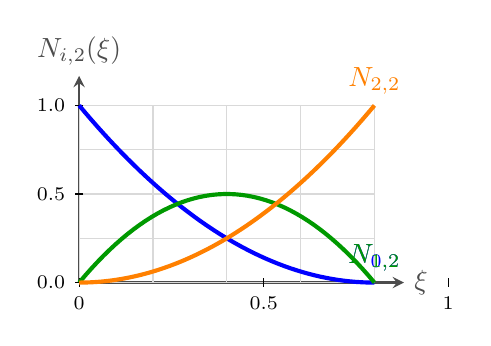
\begin{tikzpicture}[scale=0.75, >=stealth]
            \draw[->, thick, black!70] (0,0) -- (5.5,0) node[right] {$\xi$};
            \draw[->, thick, black!70] (0,0) -- (0,3.5) node[above] {$N_{i,2}(\xi)$};
            \draw[gray!30, thin] (0,0) grid[ystep=0.75, xstep=1.25] (5,3);
            % Ticks
            \foreach \x/\l in {0/0, 2.5/0.5, 5/1} {
                    \draw (1.25*\x, 2pt) -- (1.25*\x, -2pt) node[below, font=\scriptsize] {\l};
                }
            \foreach \y/\l in {0/0.0, 1.5/0.5, 3/1.0} {
                    \draw (2pt, \y) -- (-2pt, \y) node[left, font=\scriptsize] {\l};
                }
            % Plot functions
            \draw[blue, line width=1.5pt, domain=0:5, samples=50] plot (\x, {3*(1 - \x/5)^2}) node[above] {$N_{0,2}$};
            \draw[green!60!black, line width=1.5pt, domain=0:5, samples=50] plot (\x, {3*2*(\x/5)*(1 - \x/5)}) node[above] {$N_{1,2}$};
            \draw[orange, line width=1.5pt, domain=0:5, samples=50] plot (\x, {3*(\x/5)^2}) node[above] {$N_{2,2}$};
        \end{tikzpicture}
        \caption{Basis before ($\Xi = \{0,0,0,1,1,1\}$)}
        \label{fig:href_basis_before}
    \end{subfigure}
    \hfill
    \begin{subfigure}[b]{0.48\textwidth}
        \centering
        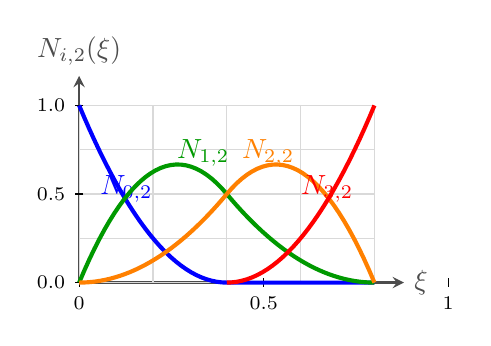
\begin{tikzpicture}[scale=0.75, >=stealth]
            \draw[->, thick, black!70] (0,0) -- (5.5,0) node[right] {$\xi$};
            \draw[->, thick, black!70] (0,0) -- (0,3.5) node[above] {$N_{i,2}(\xi)$};
            \draw[gray!30, thin] (0,0) grid[ystep=0.75, xstep=1.25] (5,3);
            % Ticks
            \foreach \x/\l in {0/0, 2.5/0.5, 5/1} {
                    \draw (1.25*\x, 2pt) -- (1.25*\x, -2pt) node[below, font=\scriptsize] {\l};
                }
            \foreach \y/\l in {0/0.0, 1.5/0.5, 3/1.0} {
                    \draw (2pt, \y) -- (-2pt, \y) node[left, font=\scriptsize] {\l};
                }
            % Plot functions after inserting knot at 0.5
            \draw[blue, line width=1.5pt, domain=0:2.5, samples=30] plot (\x, {3*(1 - \x/2.5)^2}) -- (5,0);
            \node[blue, above] at (0.8, 1.2) {$N_{0,2}$};

            \draw[green!60!black, line width=1.5pt, domain=0:2.5, samples=30] plot (\x, {3*(4*(\x/5) - 6*(\x/5)^2)});
            \draw[green!60!black, line width=1.5pt, domain=2.5:5, samples=30] plot (\x, {3*(2*(1-\x/5)^2)});
            \node[green!60!black, above] at (2.1, 1.8) {$N_{1,2}$};

            \draw[orange, line width=1.5pt, domain=0:2.5, samples=30] plot (\x, {3*(2*(\x/5)^2)});
            \draw[orange, line width=1.5pt, domain=2.5:5, samples=30] plot (\x, {3*(4*(1-\x/5) - 6*(1-\x/5)^2)});
            \node[orange, above] at (3.2, 1.8) {$N_{2,2}$};

            \draw[red, line width=1.5pt, domain=2.5:5, samples=30] plot (\x, {3*((\x-2.5)/2.5)^2});
            \node[red, above] at (4.2, 1.2) {$N_{3,2}$};
        \end{tikzpicture}
        \caption{Basis after ($\Xi = \{0,0,0,0.5,1,1,1\}$)}
        \label{fig:href_basis_after}
    \end{subfigure}

    \vspace{0.4cm}
    % Row 2: Curves and control polygons
    \begin{subfigure}[b]{0.48\textwidth}
        \centering
        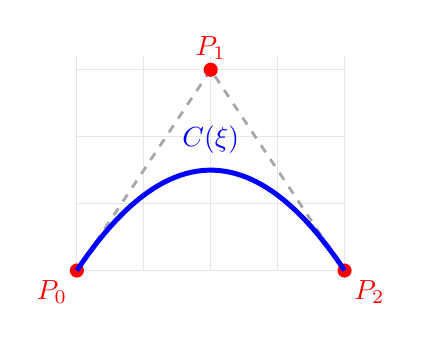
\begin{tikzpicture}[scale=0.85, >=stealth]
            \draw[gray!20, thin] (0,0) grid (4,3.2);
            % Control polygon
            \draw[gray!70, dashed, line width=1.0pt] (0,0) -- (2,3) -- (4,0);
            % Control points
            \fill[red] (0,0) circle (3pt) node[below left] {$\vect{P}_0$};
            \fill[red] (2,3) circle (3pt) node[above] {$\vect{P}_1$};
            \fill[red] (4,0) circle (3pt) node[below right] {$\vect{P}_2$};
            % Curve
            \draw[blue, line width=1.8pt, domain=0:1, samples=50] plot ({4*\x}, {6*\x*(1-\x)});
            \node[blue, above] at (2,1.6) {$\vect{C}(\xi)$};
        \end{tikzpicture}
        \caption{Curve before (3 control points)}
        \label{fig:href_curve_before}
    \end{subfigure}
    \hfill
    \begin{subfigure}[b]{0.48\textwidth}
        \centering
        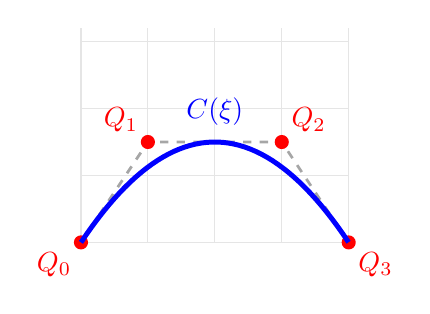
\begin{tikzpicture}[scale=0.85, >=stealth]
            \draw[gray!20, thin] (0,0) grid (4,3.2);
            % Refined control polygon
            \draw[gray!70, dashed, line width=1.0pt] (0,0) -- (1,1.5) -- (3,1.5) -- (4,0);
            % Control points
            \fill[red] (0,0) circle (3pt) node[below left] {$\vect{Q}_0$};
            \fill[red] (1,1.5) circle (3pt) node[above left] {$\vect{Q}_1$};
            \fill[red] (3,1.5) circle (3pt) node[above right] {$\vect{Q}_2$};
            \fill[red] (4,0) circle (3pt) node[below right] {$\vect{Q}_3$};
            % Curve (same shape)
            \draw[blue, line width=1.8pt, domain=0:1, samples=50] plot ({4*\x}, {6*\x*(1-\x)});
            \node[blue, above] at (2,1.6) {$\vect{C}(\xi)$};
        \end{tikzpicture}
        \caption{Curve after (4 control points)}
        \label{fig:href_curve_after}
    \end{subfigure}
    \caption{Explanatory schema of $h$-refinement (knot insertion) comparing basis functions (top) and B-spline curves (bottom) before and after inserting a knot at $\xi = 0.5$. The curve shape remains geometrically identical while the control polygon is refined.}
    \label{fig:hrefinement_basis}
\end{figure}

\subsubsection{p-Refinement (Degree Elevation)}
In $p$-refinement, the polynomial degree of the basis functions is elevated from $p$ to $p + \Delta p$ without changing the geometry or the parametric coordinates of the existing knot spans. To maintain the geometric shape exactly and preserve the continuity properties at existing knot locations, the multiplicity of all existing knots must be increased by $\Delta p$.

For a 1D curve, the new control points $\vect{P}^{\text{new}}$ are related to the original control points by a linear degree elevation operator:
\begin{equation}
    \vect{P}^{\text{new}} = \mat{T}_p \vect{P}
\end{equation}
where $\mat{T}_p$ is the degree elevation transformation matrix. Elevating the degree increases the support of each basis function and adds more control points. Unlike standard FEM where $p$-refinement introduces high-order Lagrange polynomials that can exhibit oscillatory behavior (Runge's phenomenon), IGA degree elevation preserves the non-negativity and variation-diminishing properties of B-splines.

\begin{figure}[htbp]
    \centering
    % Row 1: Basis functions
    \begin{subfigure}[b]{0.48\textwidth}
        \centering
        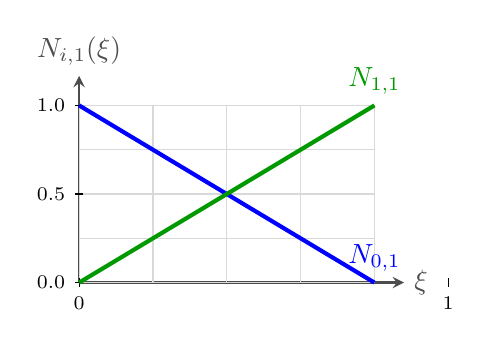
\begin{tikzpicture}[scale=0.75, >=stealth]
            \draw[->, thick, black!70] (0,0) -- (5.5,0) node[right] {$\xi$};
            \draw[->, thick, black!70] (0,0) -- (0,3.5) node[above] {$N_{i,1}(\xi)$};
            \draw[gray!30, thin] (0,0) grid[ystep=0.75, xstep=1.25] (5,3);
            % Ticks
            \foreach \x/\l in {0/0, 5/1} {
                    \draw (1.25*\x, 2pt) -- (1.25*\x, -2pt) node[below, font=\scriptsize] {\l};
                }
            \foreach \y/\l in {0/0.0, 1.5/0.5, 3/1.0} {
                    \draw (2pt, \y) -- (-2pt, \y) node[left, font=\scriptsize] {\l};
                }
            % Plot functions (Linear)
            \draw[blue, line width=1.5pt, domain=0:5, samples=2] plot (\x, {3*(1 - \x/5)}) node[above] {$N_{0,1}$};
            \draw[green!60!black, line width=1.5pt, domain=0:5, samples=2] plot (\x, {3*(\x/5)}) node[above] {$N_{1,1}$};
        \end{tikzpicture}
        \caption{Basis before ($p=1$, $\Xi = \{0,0,1,1\}$)}
        \label{fig:pref_basis_before}
    \end{subfigure}
    \hfill
    \begin{subfigure}[b]{0.48\textwidth}
        \centering
        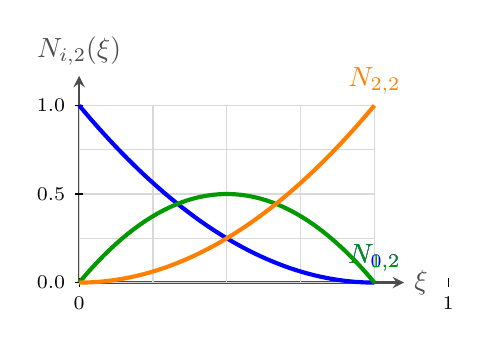
\begin{tikzpicture}[scale=0.75, >=stealth]
            \draw[->, thick, black!70] (0,0) -- (5.5,0) node[right] {$\xi$};
            \draw[->, thick, black!70] (0,0) -- (0,3.5) node[above] {$N_{i,2}(\xi)$};
            \draw[gray!30, thin] (0,0) grid[ystep=0.75, xstep=1.25] (5,3);
            % Ticks
            \foreach \x/\l in {0/0, 5/1} {
                    \draw (1.25*\x, 2pt) -- (1.25*\x, -2pt) node[below, font=\scriptsize] {\l};
                }
            \foreach \y/\l in {0/0.0, 1.5/0.5, 3/1.0} {
                    \draw (2pt, \y) -- (-2pt, \y) node[left, font=\scriptsize] {\l};
                }
            % Plot functions (Quadratic)
            \draw[blue, line width=1.5pt, domain=0:5, samples=50] plot (\x, {3*(1 - \x/5)^2}) node[above] {$N_{0,2}$};
            \draw[green!60!black, line width=1.5pt, domain=0:5, samples=50] plot (\x, {3*2*(\x/5)*(1 - \x/5)}) node[above] {$N_{1,2}$};
            \draw[orange, line width=1.5pt, domain=0:5, samples=50] plot (\x, {3*(\x/5)^2}) node[above] {$N_{2,2}$};
        \end{tikzpicture}
        \caption{Basis after ($p=2$, $\Xi = \{0,0,0,1,1,1\}$)}
        \label{fig:pref_basis_after}
    \end{subfigure}

    \vspace{0.4cm}
    % Row 2: Curves and control polygons
    \begin{subfigure}[b]{0.48\textwidth}
        \centering
        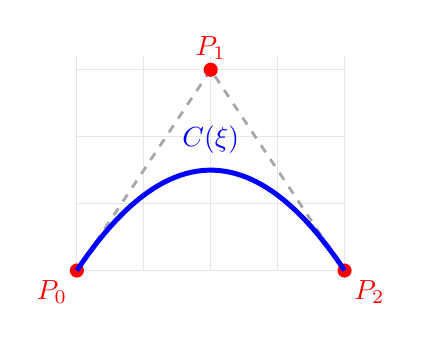
\begin{tikzpicture}[scale=0.85, >=stealth]
            \draw[gray!20, thin] (0,0) grid (4,3.2);
            % Control polygon
            \draw[gray!70, dashed, line width=1.0pt] (0,0) -- (2,3) -- (4,0);
            % Control points
            \fill[red] (0,0) circle (3pt) node[below left] {$\vect{P}_0$};
            \fill[red] (2,3) circle (3pt) node[above] {$\vect{P}_1$};
            \fill[red] (4,0) circle (3pt) node[below right] {$\vect{P}_2$};
            % Curve
            \draw[blue, line width=1.8pt, domain=0:1, samples=50] plot ({4*\x}, {6*\x*(1-\x)});
            \node[blue, above] at (2,1.6) {$\vect{C}(\xi)$};
        \end{tikzpicture}
        \caption{Curve before ($p=2$, 3 control points)}
        \label{fig:pref_curve_before}
    \end{subfigure}
    \hfill
    \begin{subfigure}[b]{0.48\textwidth}
        \centering
        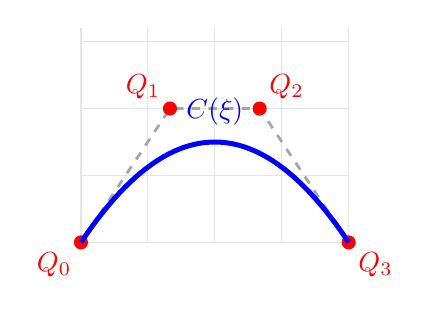
\begin{tikzpicture}[scale=0.85, >=stealth]
            \draw[gray!20, thin] (0,0) grid (4,3.2);
            % Refined control polygon (Degree elevated)
            \draw[gray!70, dashed, line width=1.0pt] (0,0) -- (1.33,2) -- (2.67,2) -- (4,0);
            % Control points
            \fill[red] (0,0) circle (3pt) node[below left] {$\vect{Q}_0$};
            \fill[red] (1.33,2) circle (3pt) node[above left] {$\vect{Q}_1$};
            \fill[red] (2.67,2) circle (3pt) node[above right] {$\vect{Q}_2$};
            \fill[red] (4,0) circle (3pt) node[below right] {$\vect{Q}_3$};
            % Curve (same shape)
            \draw[blue, line width=1.8pt, domain=0:1, samples=50] plot ({4*\x}, {6*\x*(1-\x)});
            \node[blue, above] at (2,1.6) {$\vect{C}(\xi)$};
        \end{tikzpicture}
        \caption{Curve after ($p=3$, 4 control points)}
        \label{fig:pref_curve_after}
    \end{subfigure}
    \caption{Explanatory schema of $p$-refinement (degree elevation) comparing basis functions (top) and B-spline curves (bottom) before and after elevating the polynomial degree from $p=2$ to $p=3$. The curve shape remains geometrically identical while the control polygon is enriched.}
    \label{fig:prefinement_basis}
\end{figure}

\subsubsection{k-Refinement (Order Elevation)}
A key distinguishing feature of Isogeometric Analysis is $k$-refinement, which has no direct analogue in classical Finite Element Analysis. In standard FEM, $p$-refinement always results in elements that are only $C^0$-continuous across element boundaries. In contrast, IGA allows us to increase the polynomial degree while keeping the continuity across elements as high as possible.

The $k$-refinement process is non-commutative and is performed in the following sequence:
\begin{enumerate}
    \item \textbf{Degree Elevation}: Elevate the polynomial degree from $p$ to $p + \Delta p$ on the initial coarse knot vector (which contains only the repeated boundary knots).
    \item \textbf{Knot Insertion}: Insert the desired internal knots into the elevated knot vector.
\end{enumerate}
By elevating the degree first (where the only internal knot spans are virtually non-existent or highly continuous) and then inserting knots, the resulting basis functions possess $C^{p + \Delta p - 1}$ continuity at all newly inserted internal knots. This is significantly higher than the $C^{p-1}$ continuity obtained if knot insertion is performed prior to degree elevation. The high continuity of $k$-refinement provides superior accuracy per degree of freedom, especially for structural vibration and wave propagation problems.

\begin{figure}[H]
    \centering
    \makebox[\textwidth][c]{%
        \begin{minipage}[c]{0.38\textwidth}
            \centering
            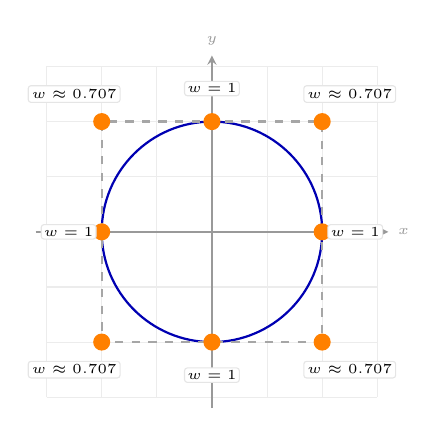
\begin{tikzpicture}[scale=1.4, >=stealth]
                % Grid
                \draw[gray!15, thin, step=0.5] (-1.5, -1.5) grid (1.5, 1.5);
                % Axes
                \draw[->, black!40, line width=0.5pt] (-1.6, 0) -- (1.6, 0) node[right, font=\tiny] {$x$};
                \draw[->, black!40, line width=0.5pt] (0, -1.6) -- (0, 1.6) node[above, font=\tiny] {$y$};

                % Perfect Circle
                \draw[blue!70!black, thick] (0,0) circle (1.0);

                % Initial control net (dashed square-like octagon)
                \draw[gray!70, dashed, thick] (1,0) -- (1,1) -- (0,1) -- (-1,1) -- (-1,0) -- (-1,-1) -- (0,-1) -- (1,-1) -- cycle;

                % Control points on axes (w=1)
                \foreach \x/\y in {1/0, 0/1, -1/0, 0/-1} {
                        \fill[orange] (\x, \y) circle (2.2pt);
                        \node[font=\tiny, fill=white, inner sep=1pt, rounded corners=1pt, draw=gray!20] at (\x*1.3, \y*1.3) {$w=1$};
                    }
                % Diagonal control points (w=0.707)
                \foreach \x/\y in {1/1, -1/1, -1/-1, 1/-1} {
                        \fill[orange] (\x, \y) circle (2.2pt);
                        \node[font=\tiny, fill=white, inner sep=1.3pt, rounded corners=1pt, draw=gray!20] at (\x*1.25, \y*1.25) {$w\approx 0.707$};
                    }
            \end{tikzpicture}
            \par\vspace{5pt}
            \small (a) Before refinement
        \end{minipage}\hfill
        \begin{minipage}[c]{0.38\textwidth}
            \centering
            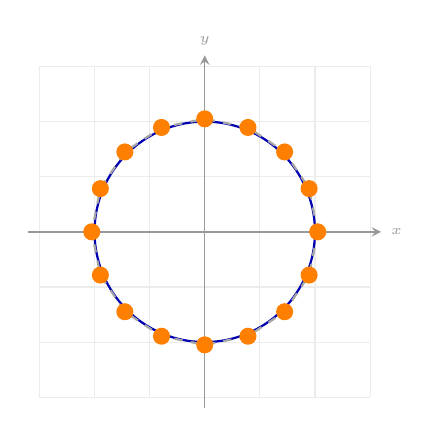
\begin{tikzpicture}[scale=1.4, >=stealth]
                % Grid
                \draw[gray!15, thin, step=0.5] (-1.5, -1.5) grid (1.5, 1.5);
                % Axes
                \draw[->, black!40, line width=0.5pt] (-1.6, 0) -- (1.6, 0) node[right, font=\tiny] {$x$};
                \draw[->, black!40, line width=0.5pt] (0, -1.6) -- (0, 1.6) node[above, font=\tiny] {$y$};

                % Perfect Circle
                \draw[blue!70!black, thick] (0,0) circle (1.0);

                % Refined control polygon (closer to circle)
                \draw[gray!70, dashed, thick] (0:1.025)
                \foreach \angle in {22.5, 45, 67.5, 90, 112.5, 135, 157.5, 180, 202.5, 225, 247.5, 270, 292.5, 315, 337.5, 360} {
                        -- (\angle:1.025)
                    };

                % Refined control points
                \foreach \angle in {0, 22.5, 45, 67.5, 90, 112.5, 135, 157.5, 180, 202.5, 225, 247.5, 270, 292.5, 315, 337.5} {
                        \fill[orange] (\angle:1.025) circle (2.2pt);
                    }
            \end{tikzpicture}
            \par\vspace{5pt}
            \small (b) After refinement
        \end{minipage}\hfill
        \begin{minipage}[c]{0.20\textwidth}
            \centering
            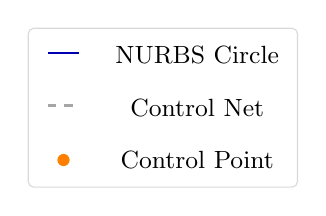
\begin{tikzpicture}[scale=0.9, ampersand replacement=\&]
                \matrix [draw=gray!30, fill=white, rounded corners=2pt, font=\small, row sep=6pt, column sep=6pt, ampersand replacement=\&] {
                    \node {\tikz[baseline=-0.5ex]{\draw[blue!70!black, thick] (0,0) -- (0.4,0);}}; \& \node {NURBS Circle};  \\
                    \node {\tikz[baseline=-0.5ex]{\draw[gray!70, dashed, thick] (0,0) -- (0.4,0);}}; \& \node {Control Net}; \\
                    \node {\tikz[baseline=-0.5ex]{\fill[orange] (0,0) circle (2.2pt);}}; \& \node {Control Point};           \\
                };
            \end{tikzpicture}
        \end{minipage}%
    }
    \caption{NURBS circle parameterization: (a) initial 8-control-point configuration with projective weights generating an exact circle, and (b) refined configuration showing the control points and net converging towards the physical circle after knot insertion.}
    \label{fig:nurbs_circle_parameterization}
\end{figure}

\begin{table}[htbp]
    \centering
    \caption{Comparative analysis of refinement strategies in Isogeometric Analysis (IGA) detailing actions, continuity, advantages, and limitations.}
    \label{tab:refinement_comparison}
    \small
    \begin{tabular}{p{2.0cm}p{1.8cm}p{1.8cm}p{3.4cm}p{3.4cm}}
        \toprule
        \textbf{Strategy}       & \textbf{Core Action}                        & \textbf{Continuity}            & \textbf{Pros (Advantages)}                                                                  & \textbf{Cons (Limitations)}                                                  \\
        \midrule
        \textbf{$h$-refinement} & Knot insertion (multiplicity $m$)           & $C^{p-m}$                      & Localized refinement capability; preserves geometry exactly; simple algebraic projection.   & Increases DOF count rapidly; doesn't elevate polynomial approximation order. \\
        \addlinespace
        \textbf{$p$-refinement} & Degree elevation                            & $C^{p-m}$ (at existing knots)  & Exponential error convergence; high accuracy per DOF; preserves geometric shape.            & Larger element stencil/bandwidth; higher computational cost per element.     \\
        \addlinespace
        \textbf{$k$-refinement} & Degree elevation followed by knot insertion & $C^{p+\Delta p - 1}$ (maximum) & Uniquely high inter-element continuity; superior accuracy per DOF; bounds Gibbs phenomenon. & No direct classical FEM equivalent; non-local basis updates.                 \\
        \bottomrule
    \end{tabular}
\end{table}

\newpage



\section{Field Approximation}
Using the isoparametric concept, the displacement field $\vect{u}(\xi, \eta) = [u(\xi, \eta), v(\xi, \eta)]^T$ is discretized using the same NURBS basis functions that represent the geometry:
\begin{equation}
    \vect{u}(\xi, \eta) = \sum_{a=0}^{N_{\text{bas}}-1} R_a(\xi, \eta) \vect{d}_a
\end{equation}
where $\vect{d}_a = [u_a, v_a]^T$ represents the displacement degrees of freedom at control node $a$, and $N_{\text{bas}} = n \times m$ represents the total number of bivariate basis functions.

\section{Global 2D Assembly \& Equations of Motion}
Applying the Galerkin discretization to the weak form yields the semi-discrete equations of motion:
\begin{equation}
    \mat{M}(\boldsymbol{\mu}) \ddot{\vect{U}} + \mat{K}(\boldsymbol{\mu}) \vect{U} = \lambda(t) \vect{F}_{\text{ext}}(\boldsymbol{\mu})
\end{equation}
where $\vect{U}$ is the global displacement vector of control variables, and $\mat{M}(\boldsymbol{\mu})$ and $\mat{K}(\boldsymbol{\mu})$ are the global mass and stiffness matrices assembled on the physical configuration $\Omega(\boldsymbol{\mu})$.

\subsection{Numerical Integration Pipeline}
Computing the stiffness matrix $\mat{K}(\boldsymbol{\mu})$ involves a multi-stage coordinate mapping pipeline to integrate the constitutive equations numerically. The step-by-step pipeline is:
\begin{enumerate}
    \item \textbf{Domain Integration}: The bilinear form is defined over the physical domain:
          \begin{equation}
              k(u^h, \delta u^h; \boldsymbol{\mu}) = \int_{\Omega^h(\boldsymbol{\mu})} \vect{\epsilon}(\delta u^h)^T \vect{\sigma}(u^h) \, dv
          \end{equation}
    \item \textbf{Element Loop}: The global integral is decomposed as a sum over elements:
          \begin{equation}
              \sum_e \int_{\Omega^e(\boldsymbol{\mu})} \vect{\epsilon}(\delta u^h)^T \vect{\sigma}(u^h) \, dv^e
          \end{equation}
    \item \textbf{Pullback to Parametric Space}: Each physical element domain $\Omega^e(\boldsymbol{\mu})$ is mapped back to the parametric element span $\Omega_p^e$:
          \begin{equation}
              \sum_e \int_{\Omega_p^e} \left( \mat{B}^T \mat{D} \mat{B} \right) |J(\boldsymbol{\xi}; \boldsymbol{\mu})| \, dv_p^e
          \end{equation}
          where $J(\boldsymbol{\xi}; \boldsymbol{\mu})$ is the parameterized Jacobian.
    \item \textbf{Parent Space Transformation}: The parametric coordinate space is mapped to the standard parent integration domain $[-1, 1]^2$:
          \begin{equation}
              \sum_e \int_{-1}^{1} \int_{-1}^{1} \left( \mat{B}^T \mat{D} \mat{B} \right) |J(\tilde{\xi}, \tilde{\eta}; \boldsymbol{\mu})| |J_{\text{parent}}| \, d\tilde{\xi} \, d\tilde{\eta}
          \end{equation}
    \item \textbf{Gauss Quadrature Summation}: The integrals are evaluated numerically using Gauss-Legendre quadrature points $\tilde{\boldsymbol{\xi}}_g = (\tilde{\xi}_g, \tilde{\eta}_g)$ and weights $w_g$:
          \begin{equation}
              \mat{K}_e(\boldsymbol{\mu}) = \sum_{g} \mat{B}^T(\tilde{\boldsymbol{\xi}}_g) \mat{D} \mat{B}(\tilde{\boldsymbol{\xi}}_g) |J(\tilde{\boldsymbol{\xi}}_g; \boldsymbol{\mu})| |J_{\text{parent}}| w_g
          \end{equation}
    \item \textbf{Global Assembly}: The element matrices are assembled using the assembly operator $\mathcal{A}_e$ or localization matrices $\mat{L}_e$:
          \begin{equation}
              \mat{K}(\boldsymbol{\mu}) = \mathcal{A}_e \left( \mat{K}_e(\boldsymbol{\mu}) \right) = \sum_e \mat{L}_e^T \mat{K}_e(\boldsymbol{\mu}) \mat{L}_e
          \end{equation}
\end{enumerate}

where the constitutive matrix $\mat{D}$ under plane stress assumptions is defined as:
\begin{equation}
    \mat{D} = \frac{E}{1 - \nu^2} \begin{bmatrix} 1 & \nu & 0 \\ \nu & 1 & 0 \\ 0 & 0 & \frac{1 - \nu}{2} \end{bmatrix}
\end{equation}
The strain-displacement matrix $\mat{B} \in \mathbb{R}^{3 \times 2N_{\text{bas}}}$ is composed of nodal blocks $\mat{B}_a$:
\begin{equation}
    \mat{B} = \begin{bmatrix} \mat{B}_0 & \mat{B}_1 & \dots & \mat{B}_{N_{\text{bas}}-1} \end{bmatrix}, \quad \text{with} \quad \mat{B}_a = \begin{bmatrix} \frac{\partial R_a}{\partial x} & 0 \\[0.3em] 0 & \frac{\partial R_a}{\partial y} \\[0.3em] \frac{\partial R_a}{\partial y} & \frac{\partial R_a}{\partial x} \end{bmatrix}
\end{equation}
The physical gradients are mapped from parametric space by solving:
\begin{equation}
    \label{eq:iga_jacobian}
    \begin{bmatrix} \frac{\partial R_a}{\partial x} \\[0.3em] \frac{\partial R_a}{\partial y} \end{bmatrix} = \mat{J}_{\boldsymbol{\xi}}^{-1} \begin{bmatrix} \frac{\partial R_a}{\partial \xi} \\[0.3em] \frac{\partial R_a}{\partial \eta} \end{bmatrix} = \frac{1}{|J_{\boldsymbol{\xi}}|} \begin{bmatrix} \frac{\partial y}{\partial \eta} & -\frac{\partial y}{\partial \xi} \\[0.3em] -\frac{\partial x}{\partial \eta} & \frac{\partial x}{\partial \xi} \end{bmatrix} \begin{bmatrix} \frac{\partial R_a}{\partial \xi} \\[0.3em] \frac{\partial R_a}{\partial \eta} \end{bmatrix}
\end{equation}

\subsection{Mesh Convergence Study}
To justify the choice of the $80 \times 40$ elements mesh discretization, a grid convergence study was conducted under a static tip bending load. These convergence numbers were computed directly using the interactive web-based simulation application. Beginning with a coarse $10 \times 5$ mesh, the grid was systematically refined using dyadic h-refinement. The vertical tip displacement $U_y$ was evaluated for each resolution. The numerical convergence results are summarized in Table \ref{tab:mesh_convergence}.

\begin{table}[htbp]
    \centering
    \caption{Mesh convergence study for the notched cantilever beam under static bending load, evaluating vertical tip displacement $U_y$ and relative convergence error.}
    \label{tab:mesh_convergence}
    \begin{tabular}{lcccc}
        \toprule
        \textbf{Resolution}     & \textbf{Elements} & \textbf{DoFs}  & \textbf{Tip Disp. $U_y$ (mm)} & \textbf{Relative Error (\%)} \\
        \midrule
        $10 \times 5$           & $50$              & $168$          & $3.538$                       & $16.51\%$                    \\
        $20 \times 10$          & $200$             & $528$          & $3.889$                       & $8.24\%$                     \\
        $40 \times 20$          & $800$             & $1,848$        & $4.083$                       & $3.66\%$                     \\
        \textbf{80 $\times$ 40} & \textbf{3,200}    & \textbf{6,888} & \textbf{4.185}                & \textbf{1.24\%}              \\
        $160 \times 80$         & $12,800$          & $26,568$       & $4.238$                       & Reference                    \\
        \bottomrule
    \end{tabular}
\end{table}

The convergence study shows that refining the mesh from $80 \times 40$ ($3,200$ elements) to $160 \times 80$ ($12,800$ elements) yields a change of only $1.24\%$ in the peak displacement, while increasing the number of equations from $6,888$ to $26,568$ (a $3.8\times$ increase). Therefore, the $80 \times 40$ discretization is selected as the operating baseline, providing an optimal balance between numerical convergence and online solve time.

The accuracy of this IGA core assembly compared to traditional Lagrangian Finite Element methods is summarized in Table \ref{tab:linear_validation}. Due to higher-order continuity across elements, IGA achieves similar accuracy to Lagrangian FEM with significantly fewer degrees of freedom.


\begin{table}[htbp]
    \centering
    \caption{Linear solution accuracy validation comparing full-order IGA degrees of freedom against fine-mesh Lagrangian FEM frameworks.}
    \label{tab:linear_validation}
    \resizebox{\textwidth}{!}{%
        \begin{tabular}{lcccc}
            \toprule
            \textbf{Mesh Setup} & \textbf{Total DoFs} & \textbf{Tip Disp. (mm)} & \textbf{Energy Norm} & \textbf{Solve Time (ms)} \\
            \midrule
            Lagrange FEM        & $12,400$            & $4.182$                 & $1.042 \times 10^5$  & $845.2$                  \\
            IGA Core            & $3,200$             & $4.185$                 & $1.044 \times 10^5$  & $142.1$                  \\
            \bottomrule
        \end{tabular}%
    }
\end{table}

\newpage

\section{Summary and Conclusion}
In this chapter, we detailed the spatial discretization of the structural domain using Isogeometric Analysis (IGA) and established the mathematical formulation of the shape-parameterized system. By utilizing the same NURBS basis functions for both geometry representation and field approximation, the exact boundary profile of the notched beam is preserved across parameter changes without mesh regeneration errors.

We derived the semi-discrete equations of motion on the physical domain $\Omega(\boldsymbol{\mu})$ and presented the numerical integration pipeline from element-level Gauss quadrature to global assembly. A mesh convergence study confirmed that the selected $80 \times 40$ discretization provides an optimal balance between accuracy and computational cost. In the next chapter, we present the reference configuration pullback mapping that addresses the domain compatibility challenges identified in Chapter~\ref{ch:theory}, before proceeding to the time integration and simulation workflows.

